%\title{Project Report}
%
%%% Preamble
\documentclass[paper=a4, fontsize=11pt]{scrartcl}
\usepackage[T1]{fontenc}
\usepackage{fourier}
\usepackage{listings}

\usepackage[english]{babel}															% English language/hyphenation
\usepackage[protrusion=true,expansion=true]{microtype}	
\usepackage{amsmath,amsfonts,amsthm} % Math packages
\usepackage[pdftex]{graphicx}	
\usepackage{url}
\usepackage{hyperref}
\usepackage{graphicx}
\usepackage{wrapfig}
\usepackage[margin=0.5in]{geometry}
\usepackage{amsmath}

%%% Custom sectioning
\usepackage{sectsty}
\allsectionsfont{\centering \normalfont\scshape}


%%% Custom headers/footers (fancyhdr package)
\usepackage{fancyhdr}
\pagestyle{fancyplain}
\fancyhead{}											% No page header
\fancyfoot[L]{}											% Empty 
\fancyfoot[C]{}											% Empty
\fancyfoot[R]{\thepage}									% Pagenumbering
\renewcommand{\headrulewidth}{0pt}			% Remove header underlines
\renewcommand{\footrulewidth}{0pt}				% Remove footer underlines
\setlength{\headheight}{3.6pt}
\date{}


%%% Equation and float numbering
\numberwithin{equation}{section}		% Equationnumbering: section.eq#
\numberwithin{figure}{section}			% Figurenumbering: section.fig#
\numberwithin{table}{section}				% Tablenumbering: section.tab#


%%% Maketitle metadata
\newcommand{\horrule}[1]{\rule{\linewidth}{#1}} 	% Horizontal rule

\title{
		\vspace{-1in} 	
		\usefont{OT1}{bch}{b}{n}
		\normalfont \normalsize \textsc{Durham Computer Science} \\ [5pt]
		\horrule{0.5pt} \\[0.4cm]
		\large  GPU, Many-core and Cluster Computing Assignment - LLLL76\\
		\horrule{2pt} \\[0.5cm]
		\vspace{-1in} 	
}

%%% Begin document
\begin{document}
\maketitle
\section{Step One}
\subsection{Results}
\begin{figure}[h]
\centering
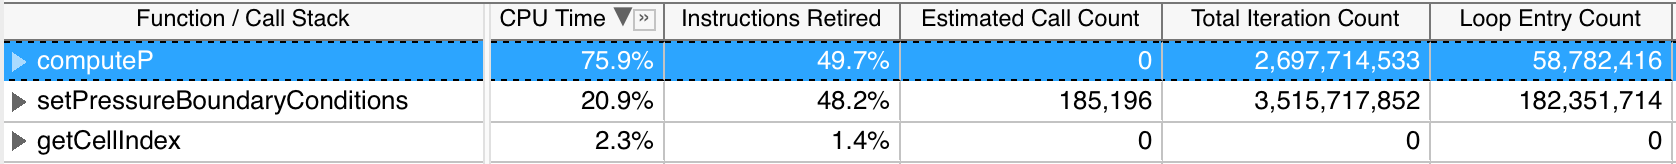
\includegraphics[width=0.75\textwidth]{one.png}
\end{figure}
\begin{figure}[h]
\centering
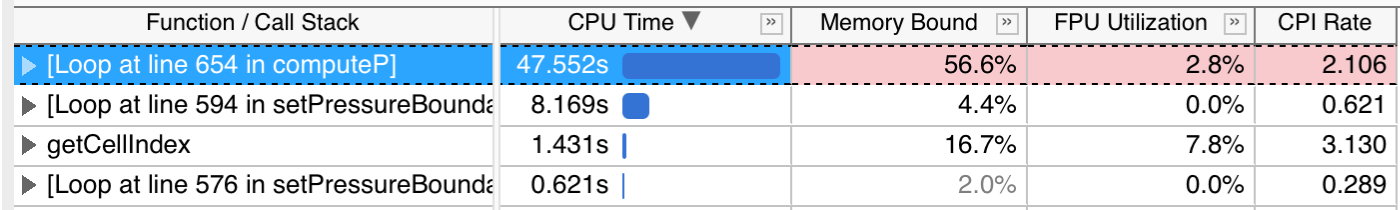
\includegraphics[width=0.75\textwidth]{two.png}
\end{figure}

This run time analysis is taken from Vtune, the analysis tools used are General Exploration, Advanced Hotspots, and HPC Performance Characterisation. It was used on a slightly altered step one, all IO has been turned off as to give an accurate representation of the computational time of the program and not add the time taken for IO. This was also run on Hamilton so the processes do not share CPU cycles or RAM with any other processes. If this was run on another system then it may have to share resources. Different compiler optimisations have been tested on this as well, -O1, -O2, and -O3 are different compiler optimisations with different severities, -O3 being the most severe and the one that was found to be the fastest in testing.
The command line parameters will also effect the run time, the first is the resolution which has a significant impact on run time as this dictates the number of cells in the simulation, the second is the time between writing a file, this has been turned off to give a pure analysis of run time, the third and final is the Reynolds number, this is the viscosity of the fluid, higher the number the more viscus the fluid, at lower numbers the run time will increase.

\subsection{Bottlenecks}

The bottle neck, as shown above is the loop in the function 'computeP'. This takes up a very large amount of the CPU Time. Another computationally significant part of the code is the function 'setPressureBoundaryConditions', whilst this does not make up as much of the CPU time as 'computeP' it is still a significant percentage. This version of the code is memory bound, the number of computations that can be done are limited by the time taken to load the data that is then used in the computation. 

\subsection{Performance Model and Predictions}

Due to the bottlenecks shown above the performance model that should be used in this case is Strong Scaling. In order to calculate the speed up in execution of this code on a higher number of processors, given as P in this instance, we use the formula \[S(P) = \dfrac{T(1)}{T(P)}\] where S(P) is the speed up of the code on P processors, T(1) is the time taken on a single processor, and T(P) is the time taken on P processors. The time taken on P processors is not known but can be calculated by Amdahl's law, given as; \[T(P) = F * T(1) + (1 - F) * \dfrac{T(1)}{P}\] where F is the fraction of serial code. We will combine the two functions to give \[ \dfrac{1}{F + \dfrac{(1 - F)}{P}} \] F in our case is any code that is not 'computeP' this makes up 24.1\% of the run time, whilst P tends to infinity. The possible speed up is 4.15. with the numbers given. 

%%%%%%%%%%%%%%%%%%%%%%%%%%%%%%%%%%%%%%

\section{Step Two}
\subsection{Description}

In step two we work to split the computational domain into smaller cubes and vectorise any showstopping parts.  A loop can be vectorised if it meets a certain criteria; it must be countable, meaning that the number of iterations must be known before we enter the loop, it must have only a single entry and a  single exit, it also must have no branching, ie no if statements. The other criteria is only inner loops, no function calls, and no internal dependencies. 

The criteria that this code breaks is the fact that it's main loop in the 'computeP' function contains branching, if this was removed then this loop could be vectorised as it meets all other criteria. We start by splitting the overall box we are working in into smaller cubes, the dimensions of these cubes is hard-coded at a single point in the code, this is easy to change. If the dimensions of the box is such that it cannot be made up of complete cubes then the code will halt. If the input variables are such that the box can be made up of a whole number of cubes then the code will move onto working out if a given cube can be vectorised, this would be the case if, out of all the cells in the given cube, none of them are part of the obstacle. If the given block contains no cells from the obstacle then it can be vectorised as in the standard realisation of the code the if statement is a check if the current cell is part of the obstacle. Thus the pre-processing for checking the status of the cells is required to allow the non-obstacle blocks to be vectorised and the blocks that do contain part of obstacle to be treated with the standard code given, using the if statement.

The stages of the vectorisation are as follows, pre-processing takes place, this will check all cells in each block and set a flag as to what is contained within the block, obstacle or not, this is stored in a boolean array. The flag that corresponds to the current block will then be used to choose which set of for loops should be used on that block, the vectorised or non-vectorised. The vectorisation is done using the standard intel SIMD pragma.

The pragma SIMD alters the order of cell propagation, the order is now block by block rather than cell by cell the overall effect is negligible. The speed up of the code however is significant as any block that does not contain a cell that is part of the obstacle is vectorised, due to the small size of the obstacle most of the blocks are vectorised and thus 'computeP', which is typically a show stopper, is significantly faster than usual. 

\subsection{Vectorisation Reports}

The vectorisation report for the unvectorised version of the code shows that the function "ComputeP" has no vectorised parts.
\begin{lstlisting}

LOOP BEGIN at gpu1.cpp(659,9)
        remark #15344: loop was not vectorized: vector dependence prevents 
        vectorization. First dependence is shown below. Use level 5 report for details
        remark #15346: vector dependence: assumed ANTI dependence 
        between _rhs[_ix+_iy*(_numberOfCellsPerAxisX+2)+(_iz*(_numberOfCellsPerA (670:25) 
        and _p[$i4] (673:13)
LOOP END

\end{lstlisting}

There are two loops that are present in step two, one that is vectorised and allowed for blocks that do not contain any parts of the obstacle to avoid the if statement in the standard loop that is unvectorised. 

\begin{lstlisting}

 LOOP BEGIN at gpu21.cpp(594,17)
		remark #15301: SIMD LOOP WAS VECTORIZED
 LOOP END

\end{lstlisting}

This is the vectorised loops vec-report, the other loop is almost identical to the loop in step one. All other parts of the report show that nothing else has been vectorised.

\subsection{Results}

These results are step one and two, they have the same command line parameters outside of grid size which is increased stepwise. They also run over the same t value.

\begin{figure}[h]
\centering
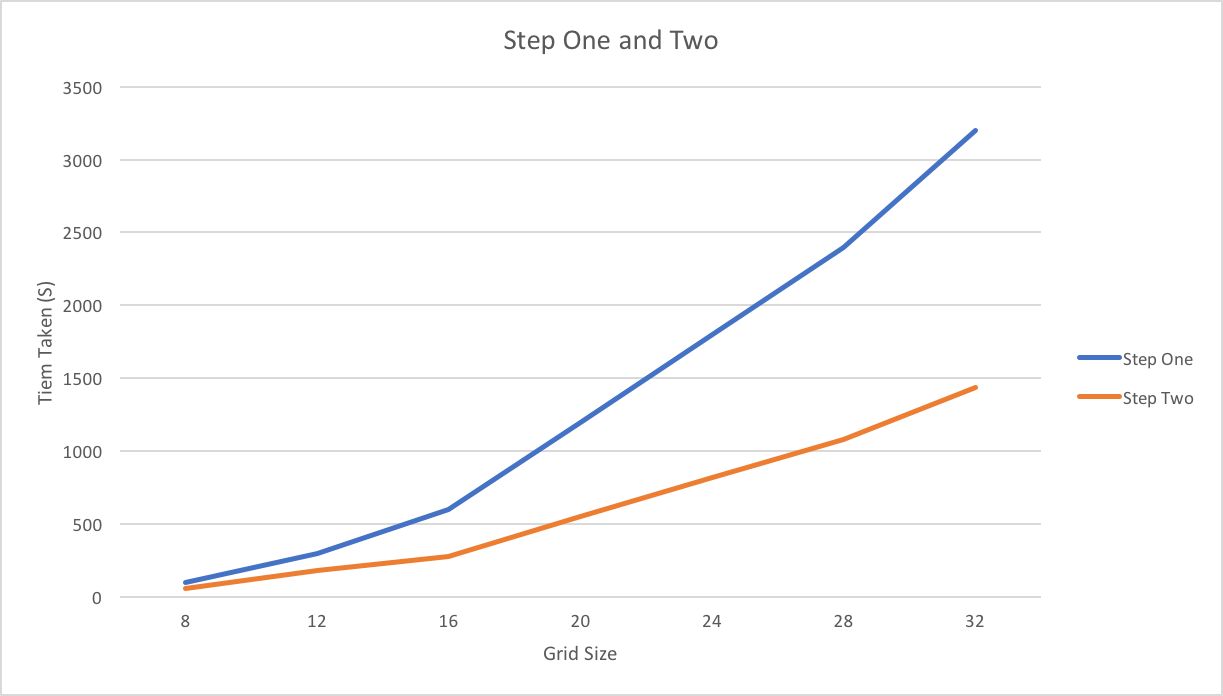
\includegraphics[width=0.5\textwidth]{StepTwo.png}
\end{figure}

%%%%%%%%%%%%%%%%%%%%%%%%%%%%%%%%%%%%%%

\section{Step Three}
\subsection{Description}

The arrays that store all values for the cells are padded in such a way that there is a layer of cells surrounding each block. In all other functions in the simulation have loops that iterate through the unpadded array, this will lead to errors unless functions that can map between the different loops and the different arrays are made. The function to map from a standard loop the the unpadded array already exists in the form 'getCellIndex', thus 'getPaddedCellIndex', 'fromHaloGetPadded', and 'fromHaloGetCellIndex' were created to convert between normal loops and halo array, halo loops and halo array, and halo loops to unpadded array respectively. At the beginning of each 'computeP' iteration the values of the padded cells are changed to the values of their corresponding non padded cell, this is done through a function 'getPaddedValues' that will take in the index of the halo cell and will return the correct value of that halo. All other functions that contain loops that used to iterate through the standard array are unchanged however the function call has been changed such that the values passed for the original array are mapped to the corresponding cell in the padded array, this is easier as a mapping function being called instead of changing all for loops in the program. Each padded block is then passed through the omp parallel pragma such that it is done in parallel using the padded values for any data that would otherwise be from a different block and would thus not allow for parallel as it would introduce data races. After this has been then we will go into a different iteration which would result in the new halo values being written from their corresponding non halo cell. Different scheduling approaches have been researched and tested, static, dynamic, and guided were all tested, in the end guided gave consistently faster results.

\subsection{Results}

\begin{figure}[h]
\centering
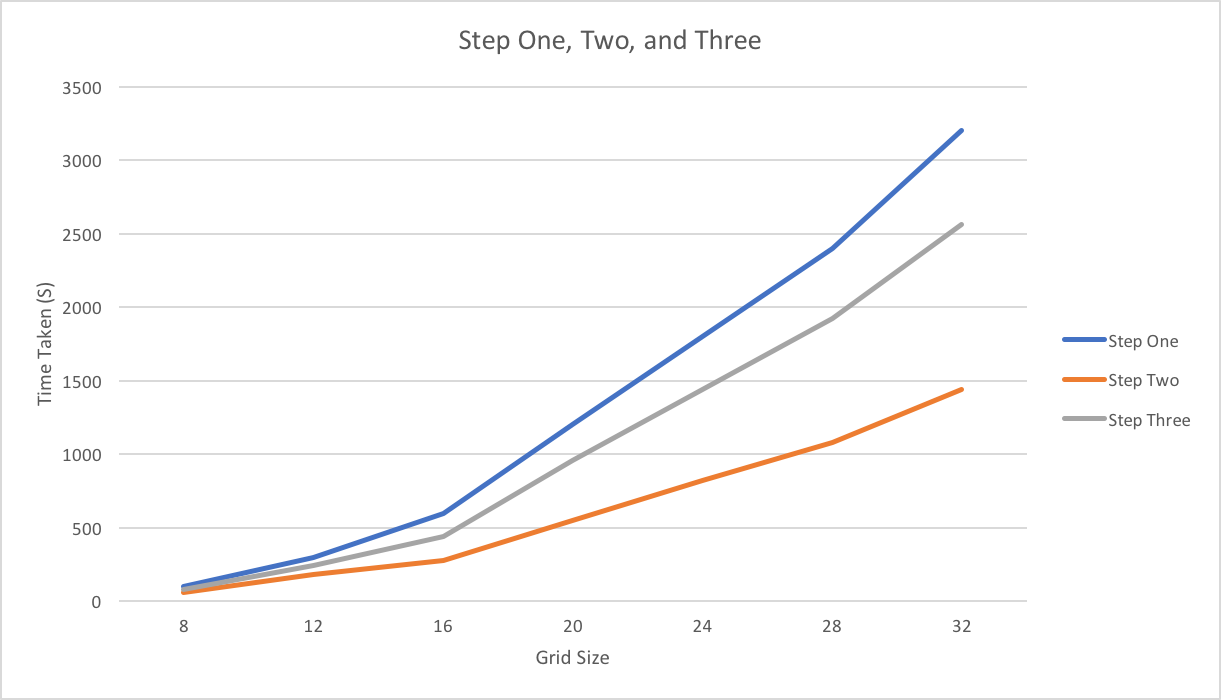
\includegraphics[width=0.5\textwidth]{StepThree.png}
\end{figure}

\subsection{Limitations}

The only seeming limitation of this approach is that of spin time, this is the overhead that is required to set up the parallel approach, in this time there is no useful computation, at least with regards to the final result, being done. This may relatively reduce when run on much larger simulations as the spin time will remain fairly constant regardless of the size of the problem being parallelised. 

%%% End document
\end{document}